\documentclass[conference]{IEEEtran}
\IEEEoverridecommandlockouts
% The preceding line is only needed to identify funding in the first footnote. If that is unneeded, please comment it out.
\usepackage{cite}
\usepackage{amsmath,amssymb,amsfonts}
\usepackage{algorithmic}
\usepackage{graphicx}
\usepackage{textcomp}
\usepackage{xcolor}
\def\BibTeX{{\rm B\kern-.05em{\sc i\kern-.025em b}\kern-.08em
    T\kern-.1667em\lower.7ex\hbox{E}\kern-.125emX}}
\begin{document}

\title{Lidar Based SLAM Algoritm\\
}

\author{\IEEEauthorblockN{1\textsuperscript{st} Ruihua Cai}
\IEEEauthorblockA{\textit{Computer Engineering Department} \\
\textit{San Jose State University}\\
San Jose, CA, US \\
ruihua.cai@sjsu.edu}
\and
\IEEEauthorblockN{2\textsuperscript{nd} Ziyuan Yan}
\IEEEauthorblockA{\textit{Computer Engineering Department} \\
\textit{San Jose State University}\\
San Jose, CA, US \\
ruihua.cai@sjsu.edu}
\and
\IEEEauthorblockN{3\textsuperscript{rd} Ruixiang Huang}
\IEEEauthorblockA{\textit{Computer Engineering Department} \\
\textit{San Jose State University}\\
San Jose, CA, US \\
ruihua.cai@sjsu.edu}
}

\maketitle

\begin{abstract}
In the field of mobile robotics, localization is a very important issue. One particularly difficult problem is how to enable a robot to determine its position in an unknown environment. Simultaneous localization and mapping (SLAM) is one way to solve this problem. Also, Lidar is the most common sensor used by mobile robots to implement SLAM. This project is intended to explore the difficulties of SLAM algorithms by implementing some simple 2D Lidar-based SLAM algorithms. This project will be simulated in Matlab to determine the accuracy and efficiency of the algorithm.
\end{abstract}

\begin{IEEEkeywords}
Lidar, SLAM, ICP
\end{IEEEkeywords}

\section{Introduction}
In real-world robot research, Simultaneous localization and mapping (SLAM) is a critical topic for helping robots to understand their location in a space and create a map for collecting and analyzing the surrounding environment. 

There are serval ways to implement SLAM on robots. Such as camera, sonar, and Lidar. Using the camera, we could use the image processing algorithm to get a graph of the current environment. Even though we could get a high-resolution image from it, due to the sensor itself doesn't provide very accurate distance data, and noise under too bright or dark conditions could affect the result. Camera-based SLAM is not common for people to research. Sonar-based SLAM is the majority applied to underwater robot SLAM. Due to the environmental issue, it could not rely on light-based sensors to perform SLAM. The best choice for underwater robots to do SLAM is based on sonar, which can handle the undercurrent in water\cite{b4}. Using Lidar is the most popular solution for solving SLAM issues. It could provide a wide range of searching angle and distance information, which is excellent for developing SLAM research. 

Since Lidar is the most common and affordable device for SLAM research. By collecting the surrounding Lidar information, we could get the outline of the surrounding area. Due to the advantages of Lidar, which include the distance information, we could determine the distance between the robot and the wall or obstacles around the robot. In this project, we will develop two kinds of SLAM algorithms without the data of odometry. The first algorithm is based on the prediction robot’s movement to match the similarity between the previous scan and the current scan result. If the robot could match the pattern of the scan result, we can say the robot moved in this direction and distance. The second algorithm is based on the Iterative Closest Point (ICP) algorithm. By comparing the closest point shifting between the previous scan and the current scan, we could get a vector shifting that is suitable for most of the points, and this vector is the movement of the robot. 

\section{Related Work and Background Material}
By studying Wolfgang \& Damon\cite{b1} and John \& John\cite{b4}'s article, we have a more comprehensive understanding of the different sensor-based robot SLAM algorithms and how it benefits human life. This involved our interest in researching different kinds of SLAM approaches.  In Shan's article \cite{b2}, he demonstrates a way to implement SLAM by combining multiple sensor data and using the Extended Karmal Filter (EKF) to perform sensor fusion for calculating SLAM. We study how this author uses 2D-Lidar to collect the surrounding environment data and understand the basic theory of localization. Finally, from Shaofeng \& Jingyu's article \cite{b3}, we found another approach to implementing robot SLAM based on Lidar. Through the above research and study, these articles gave us basic knowledge and direction about how to implement SLAM into our project.

\section{Technical  approach}
\subsection{Pattern Match SLAM}
The pattern match algorithm is our own design of the SLAM algorithm. We want to find the current position of the robot by assuming the displacement amount. Whenever a new scan is obtained, the program first speaks the result of the scan through a coordinate transformation to obtain a matrix with a set resolution. Each point in the matrix that has a lidar mapped to it is set to 1, and points that are not mapped are set to 0. We then convert the current scan by traversing the possible displacements and comparing the difference with the previous result. Then we obtain the difference between the two matrices by summing the absolute values of the difference matrix. By recording the displacement of the matrix with the smallest difference, we obtain the displacement between the robot this time and the last received result. Then by adding the previous coordinates to the current displacement, we obtain the correct coordinates. Since the first step of the algorithm is to obtain a matrix that can be calculated quickly by reducing the resolution of the scan. The accuracy of the algorithm gets better as the resolution increases, but because all possible displacements are calculated each time, the efficiency of the algorithm becomes slower as the resolution increases. To solve this problem, we add the parameter search distance to limit the number of displacements that the algorithm traverses. However, this also limits the distance of a single displacement of the robot, which can cause the algorithm to lose track if the robot is displaced too far.

\subsection{Iterative Closest Point SLAM}
In order to be able to reduce the number of operations to calculate the current coordinate locations, we want to ensure that the algorithm maintains a stable coordinate determination under the high-accuracy radar detection information. The first algorithm, it requires a lot of comparison cycles to find the current position, which will take a lot of time to compute, especially in a high-precision environment. To solve this problem, we intend to try a mathematical approach. Thanks to the inspiration of Nearest Neighbor Processing (NNP), we learned about the Iterative closest point (ICP) algorithm, and we intend to apply it to our SLAM. In ICP, it will convert the information from the current radar scan and the previous radar information into two sets of coordinate positions of the obstacle. 
\begin{equation}
    CurrPos = PrePos + [\sum_{i=1}^{n}(Vector_i)]/n\label{eqICP}
\end{equation}

Afterward, by overlapping the two sets of data while removing the unchanged part and keeping the moving part. The position of the obstacle that has changed before and after the movement can be obtained. Moreover, based on the current radar information, each node in the current set will find the nearest node in the previous radar information. Simultaneously it will save the angle and distance difference between each node and its nearest neighbor in a new array. Through this method, we can obtain an array containing the approximate direction and distance of each node. However, the data at this point contains a lot of noise information in order to reduce the impact of noise on the data. This algorithm will be done by finding the top five sets of plural data with the largest percentage in the array and getting the vector information of their average values. Therefore, the relative direction and distance of the overall movement will be estimated to get the current position

\section{Results Analyze}
To test the performance between the two algorithms in a practice situation, we created a simulated 3d environment using Matlab's built-in editor to test the robot's localization capabilities. In the environment, we placed a certain number of obstacles and set the robot's travel path, obtained a simulated radar signal from the robot's current location, and used both algorithms to estimate the robot's position. While we can adjust the precision to expand the scanning range and accuracy of the radar, in this way, we can test the algorithm in the ideal environment.


\subsection{Figures and Tables}
By testing the two algorithms in different resolution setting, we obtained two sets of data and made them into a table. In the first set of data \ref{RuntimeFig}, we compare the time consumed by the algorithm at different accuracies by using Matlab's built-in timing function, showing that the first algorithm shows an exponential increase in running time as the scanning accuracy increases. In contrast, the second algorithm can still maintain a very fast computational power under high-precision scanning.

\begin{figure}[htbp]
\centerline{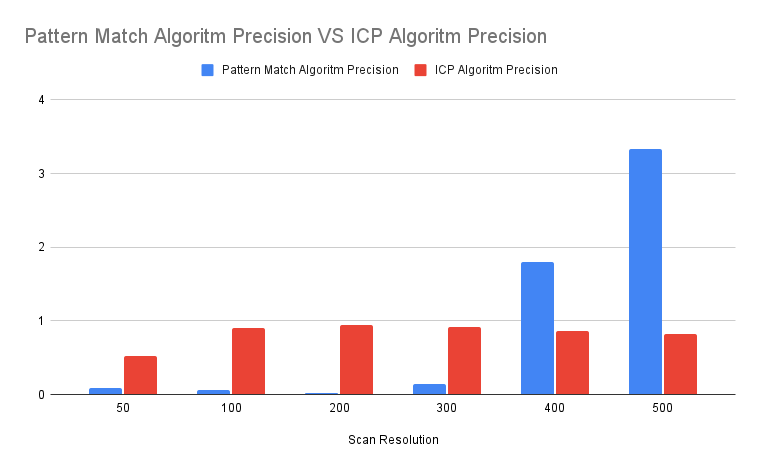
\includegraphics[width=\linewidth]{../result/Pattern_Match_Algoritm_Precision_VS_ICP_Algoritm_Precision.png}}
\caption{Pattern Match Algoritm Precision VS ICP Algoritm Precision}
\label{PrecisionFig}
\end{figure}

\begin{equation}
\Delta E = \sqrt{\overline{X_e}^2 + \overline{Y_e}^2}\label{eqError}
\end{equation}
In the second set of data \ref{PrecisionFig}, we can get the precision of the algorithm in different environments by using the formula \eqref{eqError} to compare the precision of the algorithm at different accuracies. The first algorithm can be found to maintain a very good precision at a resolution less than or equal to 300, while the precision is significantly out of tune at a resolution greater than 400. On the other hand, the overall accuracy of the second algorithm does not vary much. Although the accuracy is much less than the first algorithm in the case of low resolution, it can still maintain a stable operation under high precision.

\begin{figure}[htbp]
\centerline{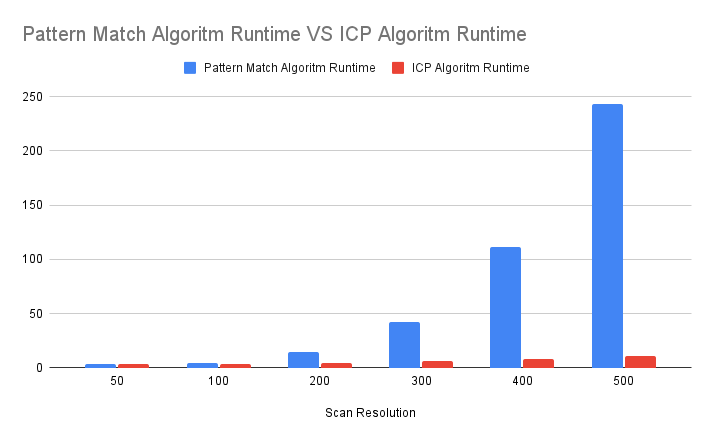
\includegraphics[width=\linewidth]{../result/Pattern_Match_Algoritm_Runtime_VS_ICP_Algoritm_Runtime.png}}
\caption{Pattern Match Algoritm Runtime VS ICP Algoritm Runtime}
\label{RuntimeFig}
\end{figure}


\section{Conclusion}
In general, the Pattern matching algorithm can have better accuracy among the two algorithms we implemented, but the computation time is too long in the case of high clarity. The ICP algorithm is able to obtain the position quickly but with poor accuracy. Both algorithms have their advantages and disadvantages, but neither is the best solution. Also, our test environment was conducted virtually. It is expected that our algorithm will perform worse in a realistic environment. However, the algorithm practice gave us a better understanding of how SLAM algorithms are implemented. As Shan mentioned in his paper, the purely 2D Lidar-based SLAM algorithm has a lot of limitations\cite{b2}. In the future, we hope to achieve more accurate SLAM positioning by adding filtering algorithms and other sensors.

\begin{thebibliography}{00}
\bibitem{b1} W. Hess, D. Kohler, H. Rapp and D. Andor, "Real-time loop closure in 2D LIDAR SLAM," 2016 IEEE International Conference on Robotics and Automation (ICRA), 2016, pp. 1271-1278, doi: 10.1109/ICRA.2016.7487258.
\bibitem{b2} S. Huang, H.-Z. Huang, Q. Zeng, and P. Huang, "A Robust 2D Lidar SLAM Method in Complex Environment", Photonic Sensors, vol. 12, no. 4, p. 220416, Apr. 2022.
\bibitem{b3} S. Wu and J. Lin, "A novel SLAM framework based on 2D LIDAR", Journal of Physics: Conference Series, vol. 1650, no. 2, p. 22104, 2020.
\bibitem{b4} J. Folkesson and J. Leonard, "Autonomy through SLAM for an underwater robot", in Robotics Research, Springer, 2011, pp. 55-70.
\end{thebibliography}
\vspace{12pt}

\end{document}
